\documentclass[atiam, article]{rapport} % draft, phelma_black, phelma_normal, kit_de, kit_en, phelma_old


\doctitle{Traitement de signal non linéaire, filtre Moog}
\title{Auto-oscillations des instruments de musique : modèles, simulations, descripteurs et cartographies}
\titleheader{PAM - Auto-oscillations des instruments de musique}
\titleone{Projet et Applications Musicales}
\titletwo{Rapport bibliographique}
\titlethree{}
\author{C. Fernandez, P. Jardin, V. Piton, H. Audas, P. Estève, B. Quiédeville} % Authors for the header
\autpage{ % Authors for the title page
  \begin{tabular}{l}
    Paul Estève \\
    Charlotte Fernandez\\
    Pharoah Jardin\\
    Victor Piton\\
    Hugo Audas\\
    Benjamin Quiédeville
  \end{tabular}
}
\supervisor[Encadrants : ]{\\Thomas Hélie\\Christophe Vergez}
% \supervisorMail{}
\serie{ATIAM 2023/2024}
\date{\today}
\addbibresource{report/biblio.bib}
% \bibliographystyle{plain}
% \bibliography{report/biblio}

\usepackage{comment}

\begin{document}

\maketitle

\tocpage

\section*{Introduction}
L'objectif de ce projet est de construire et contrôler des instrument auto-oscillants. Pour répondre à cet objectif, il est nécessaire de (1) modéliser le fonctionnement des instruments de musique auto-oscillants, (2) d'étudier les méthodes de résolution des équations non-linéaires issus des modèles physiques identifiés permettant une synthèse sonore et un contrôle de ces modèles en temps réel, et (3) de définir des décideur et des paramètres de contrôle des modèles numériques d'instruments. Ces trois questions font l'objet individuellement de nombreux travaux de recherche actuelle. Notre travail propose une étude succincte de la littérature existante sur ces différents sujets. 


\section{Modèles physiques pour les instruments auto-oscillants}\label{sec:models physiques}
Dans cette section nous allons présenter les principaux formalismes utilisés pour modéliser les instruments auto-oscillants tels que les clarinettes, cuivres, violons, etc. 
On sépare la modélisation de ces instruments en deux parties : la modélisation du résonateur et la modélisation de l'excitateur qui forment un système couplé. 

\subsection{Modélisation des résonateurs}
\subsubsection{Modélisation modale}
La modélisation des résonateurs par une approche modale, repose sur la décomposition de l'impédance d'entrée de l'instrument comme une somme de contributions d'oscillateurs à un degré de liberté. (\cite{missoum_explicit_2014} partie 3 du papier). 

On peut ainsi écrire l'impédance à l'entrée de l'instrument comme : 
\begin{equation}
    Z_e(\omega) = \frac{P_e(\omega)}{U_e(\omega)} = j\omega\sum_{n}\frac{F_n}{\omega_n-\omega+j\omega\omega_n/Q_n}
\end{equation}
Avec $F_n$ : l'amplitude , $\omega_n$ la pulsation propre, $Q_n$ le facteur de qualité du mode n et $\omega$ la pulsation. 

En isolant chaque mode, nous obtenons une équation différentielle qui permet de décrire la dynamique de l'instrument. Cette équation n'est cependant vraie que pour le mode considéré, dans le cas où on n'utilise que le premier mode, cette approche est une approche uniquement valable pour décrire l'instrument en basses fréquences. 

\subsubsection{Modélisation d'un résonateur par un guide d'ondes}

\paragraph{Modèle général}\label{sec:guide}

Un modèle plus simple utilisé par McIntyre et al. \cite{mcintyre_oscillations_1983} et Maganza et al. \cite{maganza_bifurcations_1986} repose sur la décomposition de la variable potentiel $q(t)$ et de la variable flux $f(t)$ en deux : (1) une partie progressive $q_o(t)$ ; une partie rétrograde $q_i(t)$, reliées entre elles par une relation de réflexion $q_i(t)=r(t)*q_o(t)$. De plus, $q(t)$ et la variable de flux $f(t)$ sont reliées par la relation linéaire d'impédance.

 
\paragraph{Application à une cavité cylindrique}

\cite{maganza_bifurcations_1986} développe le modèle décrit en \ref{sec:guide} dans le cas précis de la clarinette en raison de sa simplicité : géométrie cylindrique de la cavité, excitation faite par une anche simple. L'étude est limitée aux ondes planes harmoniques.% Nous définissons le coefficient de réflexion $R(x,\omega)$, puis la relation de linéarité entre $P(x,\omega)$ et $U(x,\omega)$ s'obtient par la relation d'impédance. Le lien entre pressions et vitesses en tout point du guide doit être exprimé. Pour ce faire, nous utilisons un formalisme similaire à celui des lignes de transmission en électricité : définir une matrice de transfert liant la pression et la vitesse acoustique en deux points du guide d'ondes.


\subsubsection{Analogie avec le résonateur du violon}

Dans \cite{ollivier_idealized_2004} l'analogie entre le résonateur des instruments à vents et le résonateur des instruments à cordes frottées comme le violon est faite. Pour un instrument à cordes frottées, le résonateur est constitué de l'ensemble $\left\{ corde + chevalet + caisse\right\}$. Les ondes propagatives sont supposées réfléchies aux limites de la corde selon différentes hypothèses.

\begin{itemize}
  \item Un premier modèle non dissipatif est tel que la réflexion $r(t)$ aux limites (doigt ou chevalet) est simplement une fonction du retard $\tau$ qui correspond au temps de trajet des ondes sur une distance de corde comprise entre le doigt et le chevalet $r(t)=-\delta(t-\tau)$
  \item Un second modèle dissipatif, dit de Raman, ajoute simplement un amortissement $\lambda < 1$ au modèle précédent: $r(t)=-\lambda \delta(t-\tau)$
  \item Un troisième modèle plus réaliste du point de vue de la dispersion  considère une largeur temporelle finie pour le coefficient de réflexion. Ce modèle n'est cependant pas simple à résoudre analytiquement.
\end{itemize}

Finalement, le modèle simple de réflexion non dissipative permet d'exprimer l'admittance d'entrée du résonateur dans le domaine fréquentiel, de manière analogue aux instruments à vent, comme la rapport $Y=v/f$ de la vitesse relative entre la corde et l'archet, et de l'effort appliqué par l'archet sur la corde.

$$Y=v/f=jY_c(cot(kL_a)+cot(kL_b))$$

Où $L_a$ et $L_b$ représentent les deux longueurs de corde séparées par la position du doigt, $Y_c$ est l'impédance caractéristique de la corde et $k$ le nombre d'onde.


\subsection{Modélisation des excitateurs}

\subsubsection{Cas général d'un excitateur non-linéaire}\label{subsubsection:excitateur_cas_général}

\cite{mcintyre_oscillations_1983} et \cite{maganza_bifurcations_1986} proposent un modèle général d'excitateur, reliant les variables de flux $f$ et de potentiel $q$ : $f=F(q)$, où $F$ est une fonction non-linéaire.

\subsubsection{Exemple pour la clarinette}
Un modèle de clarinette est proposé dans \cite{missoum_explicit_2014} et dans \cite{chaigne2008acoustique} (chap. 9 section 2.6). Il repose sur la modélisation de l'excitation de l'instrument par le débit acoustique en entrée du bec en fonction de la pression. Cette modélisation est un cas particulier du cas général \ref{subsubsection:excitateur_cas_général}. 
Dans ce formalisme, le débit d'entrée dans le bec de la clarinette adimensionnée est défini comme : \\

\begin{equation}
    u(t) = \begin{cases}
    \zeta(1-\gamma+p)\sqrt{|\gamma-p|}sgn(\gamma-p),& \text{si }\gamma-p\geq 1\\
    0,              & \text{sinon}
\end{cases}
\end{equation}

avec $\zeta$, une paramètre adimensionné régi par l'ouverture de l'anche, $\gamma$ un paramètre de la pression dans la bouche adimensionnée. En faisant un développement limité de $u(t)$, on obtient une équation différentielle de type Van der Pol \cite{chaigne2008acoustique}.

\subsubsection{Analogie avec l'archet du violon}

Dans \cite{ollivier_idealized_2004} l'analogie entre l'excitateur des instruments à anche et l'archet des instruments à cordes frottées comme le violon est également faite. 

Le phénomène non linéaire de l'excitation des cordes par un archet est le "collé-glissé". Il s'agit d'une alternance entre des phases d'adhérence entre les cordes et le crin de l'archet et des phases de non adhérence. Un modèle idéalisé de ce phénomène permet d'exprimer l'effort transmit à la corde par l'archet de la manière suivante:

$$f(\Delta v) = F_b[\mu _d +(\mu_s - \mu_d) \phi(\Delta v)],$$

où $\Delta v$ est la vitesse relative entre l'archet et la corde, $\mu _d$ et $\mu _s$ sont respectivement les coefficients de friction dynamique et statique et $\phi(\Delta v)$ est une fonction qui vaut $1$ si $\Delta v = 0$ et $0$ si $\Delta v = -\infty$. $F_b$ est la force de jeu subie par l'archet.

La transition entre l'état collé et l'état glissé est donné par la valeur $F_{max} = F_b \mu_s$ de l'effort transmis à la corde par l'archet, analogie de la valeur de pression limite qui permet de garder l'anche fermée.

Enfin, la comparaison entre l'effort $F_b$ et le débit de jeu dans les instrument à vent permet de compléter l'analogie entre les deux excitateurs anche et archet.

\begin{comment}
    \subsection{Discussions concernant les différents modèles physiques d'instruments auto-oscillants}
    Intérêt et inconvénient de chaque méthodes : 
    - modale : approche que sur quelques modes en général, donc approche BF , equation differentielle à résoudre, 
\end{comment}

\section{Méthodes de résolution des équations non linéaires}\label{sec : méthode de résolution des equations non linéaires}

\subsection{Méthode graphique de résolution pour les modèles à guide d'onde}

Le système final présenté par \cite{mcintyre_oscillations_1983} et \cite{maganza_bifurcations_1986} est composé de deux équations :

\begin{equation}
    \left\{\begin{split}
        &f(t)=F(q_o(t)+q_i(t))\\
        &q_o(t) - q_i(t) = Zf(t)
    \end{split}
    \right.
\label{eq:sys_guide}
\end{equation}

Décomposer les variables de débit et de pression en une partie progressive et une partie rétrograde permet une méthode de résolution graphique, sans avoir à tenir compte de délais multiples.
On note, avec les notations de Maganzana et al. \cite{maganza_bifurcations_1986}, $-q_i(t) = \mathcal{F}[-q_i(t-T)]$, où $T=2L/c$ est le temps d'un aller-retour de l'onde dans le résonateur.


% \begin{figure}
%     \centering
%     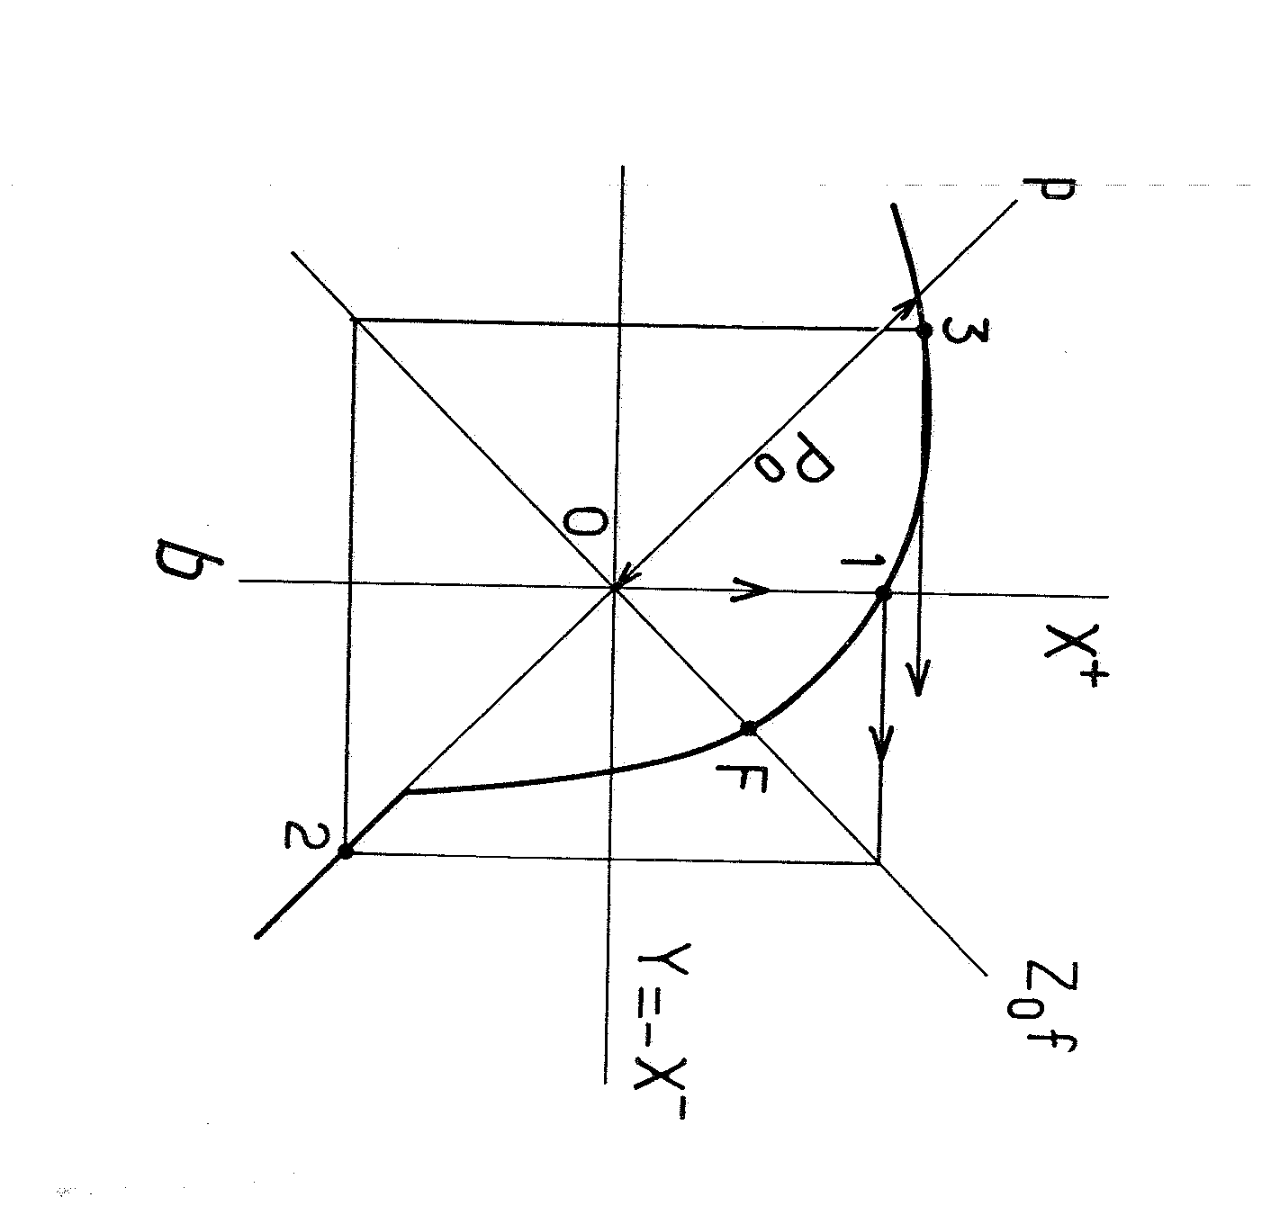
\includegraphics[angle=90,scale=0.3]{report/Images/po_pi.png}
%     \caption{Méthode de résolution graphique du système d'équations \ref{eq:sys_guide} associé au modèle du guide d'ondes. Les solutions sont trouvées dans le plan $-q_i$,$q_o$ (ici $-x^-$,$x^+$). La courbe en gras correspond à $f = F(q_o+q_i)$, pour un $f$ donné. La courbe croissante correspond à l'équation $q_i=Rq_o$. Le(s) point(s) d'intersection entre ces deux courbes donne la solution stationnaire du système. La courbe décroissante $q_o=q_i$ correspond à un flux nul et donc à l'absence de son (crédit : \cite{maganza_bifurcations_1986}).}
%     \label{fig:po_pi}
% \end{figure}

% Les solutions sont trouvées dans le plan $-q_i$,$q_o$ (ici $-x^-$,$x^+$). La courbe en gras correspond à $f = F(q_o+q_i)$, pour un $f$ donné. La courbe croissante correspond à l'équation $q_i=Rq_o$. Le(s) point(s) d'intersection entre ces deux courbes donne la solution stationnaire du système. La courbe décroissante $q_o=q_i$ correspond à un flux nul et donc à l'absence de son. 

% Supposons une situation de départ $(f,q_i,q_e) = 0$. Si $f(t)$ est la fonction échelon, alors à $t\geq 0$, $q_o$ augmente. L'onde acoustique n'ayant pas encore été réfléchie par l'extrémité du guide, $q_i=0$ et $q_o=F^{-1}(f)$ : nous sommes au point (1). Une fois que l'onde réfléchie arrive à l'entrée du guide, sa valeur est $q_i=Rq_o$ (image du point (1) par rapport à la courbe croissante). $f$ étant constante, $q_o$ varie de sorte à être sur la courbe non linéaire : nous sommes au point (2). De même, on trouve $q_i$ par l'image du point (2) par la courbe $q_i=Rq_o$ et on trouve $q_o$ de sorte à être sur la courbe non linéaire (point (3)). Cette méthode itérative permet de connaître la position du point $q_o,q_i$ à chaque pas de temps. On note, avec les notations de Maganzana et al. \cite{maganza_bifurcations_1986}, $-q_i(t) = \mathcal{F}[-q_i(t-T)]$, où $T=2L/c$ est le temps d'un aller-retour de l'onde dans le résonateur.

Remarquons que le point d'équilibre n'est pas nécessairement stable ou attractif. Il est donc possible, en fonction de l'allure de la courbe non-linéaire, d'obtenir des comportements oscillants (et donc la production de son, ondes carrées pour le fondamental) ou chaotiques. %(intersection entre la courbe non-linéaire et la courbe croissante)

L'étude de $\mathcal{F} \circ \mathcal{F}$ peut permettre d'étudier l'apparition de sous-harmoniques. Ceux-ci sont peu fréquemment observés pour des clarinettes, car ils correspondent à une très faible région de paramètres de pression et position de l'anche au repos pour les anches utilisées couramment. Ces notes, appelées sous-harmoniques, sont cependant un phénomène mieux connu chez les instruments à cordes frottées, en particulier dans le régime transitoire \cite{kergomard_instruments_1997}, \cite{mcintyre_oscillations_1983}.

% Petite mention des harmoniques supérieurs, obtenus avec le trou de registre mais qu'on a pas trop vu dans la biblio
Dans un instrument à vent, l'ouverture d'un trou de registre vient souvent permettre de jouer les harmoniques supérieurs (quinte ou octave). Une fois dans ce registre, fermer le trou de registre ne provoque le plus souvent pas un retour au fondamental.
Kergomard résume ainsi que pour un instrument à vent, \og la succession montante s’obtient en changeant les conditions initiales, la succession descendante en changeant les paramètres\fg \cite{kergomard_instruments_1997}.

\subsection{Solveurs explicites} \label{sec:solveurs}

Une première méthode que l'on trouve dans la littérature pour étudier les équations non linéaires de type van der Pol est la linéarisation de ces équation. Cette approche permet d'étudier les équilibres du système et la stabilité de ses solutions. Cependant, cette approche est insuffisante pour étudier de façon plus complète les instruments de musique. 

Une autre approche consiste à résoudre ces équations à l'aide de solveurs explicites. L'équation qui régis le fonctionnement du modèle de clarinette présenté par Missoum et al. \cite{missoum_explicit_2014} (section3.2 numercial implemention) utilise un solveur explicite de type ODE15s de la suite Matlab. 

\subsection{Discrétisation des modèles simples, analogie entre les instruments à anche et les instruments à cordes frottées}

Dans Ollivier et al. \cite{ollivier_idealized_2004}, les solutions oscillantes au point de couplage doivent vérifier à la fois les équations de l'excitateur non linéaire et les équations du résonateur. 

Pour les instruments à anche et pour les instruments à cordes frottées les équations au point de couplage peuvent être discrétisées et apportent une allure de solutions recherchées. Ces solutions sont des oscillations à "deux étages" correspondant à des signaux en créneaux modulables en fonction des différents paramètres de contrôle du musicien.


\subsection{Méthodes en temps réel}

Une des finalités de cette étude serait d'implémenter les techniques évoquées dans un logiciel fonctionnant en temps réel.
Ce logiciel serait pilotable par l'intermédiaire d'un clavier MIDI ainsi que d'une tablette graphique  pour modifier les différents paramètres de jeux de l'instrument virtuel.

Une implémentation temps réel présente des contraintes supplémentaires de coût computationnel et de causalité de l'algorithme de synthèse choisi. 
En effet, les algorithmes basés sur une résolution itérative du système d'équation différentielles (comme Newton-Raphson ou les solveur explicites présentés en \ref{sec:solveurs}) présentent des complexités de calcul trop élevées pour générer chaque échantillon, le rendant potentiellement inutilisable dans une application temps réel au delà d'un seuil de complexité du système d'équations.

La synthèse par guide d'ondes \cite{smith1987music} présentée en \ref{sec:guide} propose enfin de modéliser les différentes parties de l'instrument par des lignes à retard et des jonctions dispersives.
Cette méthode de synthèse présentes les avantages de réduire les temps de calcul à chaque échantillon à générer en échange d'un coût mémoire potentiellement supérieur.

Ces solutions temps réel pourront être implémentées en utilisant des outils tel \textit{MaxMSP}, \textit{Pure Data} permettant une bonne interactivité ou encore \textit{Faust} pour une approche fonctionnelle de la programmation audio.

\section{Cartographie et descripteurs}
\subsection{Cartographie}
Les instruments auto-oscillants, en raison de l'importance des non-linéarités dans leur fonctionnement, possèdent une très grande diversité de modes de jeu. Ainsi dans une optique de compréhension du fonctionnement de ces instruments mais également de simulation, étudier les relations entre paramètres de jeu/ contrôle, paramètres de facture et modes de jeux est primordiale et fait l'objet de nombreuses recherches. 

Une méthode de cartographie présentée par Missoum et al. \cite{missoum_explicit_2014}, repose sur des SVM (pour \textit{Support Vector Machines}). 
% Un SVM définit une frontière explicite entre des éléments appartenant à deux classes définies comme $+1$ ou $-1$. 
% La frontière entre ces deux groupe est définie comme \cite{missoum_explicit_2014} : 
% \begin{equation}
%     s(\textbf{x}) = b + \sum_{i=1}^{N}\lambda_iy_iK(\textbf{x}_i,\textbf{x}) = 0 ,
% \end{equation}
% où N est le nombre d'échantillons à classifier $\textbf{x}_i$, $b$ est le biais, $\lambda_i$ est le multiplicateur de Lagrange et $K$ est la fonction noyau. 
Les SVM sont des méthodes utilisées et adaptées pour des systèmes hautement non linaires, et permettent d'utiliser plusieurs critères de classification en n'utilisant qu'un classifieur. Il est non sensible aux discontinuités(important pour pouvoir étudier les changement de régimes/registres) et est computationnellement très efficace. Cet article présente également l'intérêt d'associer à un classifieur SVM une méthode d'échantillonnage  adaptatif, issue de \cite{basudhar2010improved}. 

La combinaison de ces deux éléments permet d'améliorer l'efficacité computationnelle et pour un même nombre de calcul d'aboutir à des résultats plus précis. La méthode présentée dans \cite{missoum_explicit_2014} est validée sur un modèle de clarinette simplifié, correspondant au modèle physique de clarinette présenté dans \ref{sec:models physiques}.


\subsection{Descripteurs}

Pour implémenter la méthode des \textit{Support Vector Machine}, il est nécessaire de choisir une liste de descripteurs permettant de caractériser les différents modes de fonctionnement de l'instrument. 
Le critère choisi et utilisé dans \cite{missoum_explicit_2014} est le fait que l'instrument produise un son ou non. 
Il est aussi possible d'utiliser un descripteur pour caractériser le son produit et déterminer des régimes particuliers de fonctionnement. 
Gibiat \cite{gibiat_phase_1988} propose d'utiliser la représentation en espace des phases accompagnée d'une analyse de Fourier pour détecter le comportement multiphonique d'une clarinette. 
En effet, la représentation dans l'espace des phases propose une lecture et une détection plus simple du doublement de période apparaissant pour des conditions de jeu particulières ces observations sont illustrées en figure \ref{fig:gibiat-double-period} tirée de \cite{gibiat_phase_1988}. 
Cette représentation est obtenue en traçant l'évolution des degrés de liberté du système ou dans le cas d'une réduction à un degré de liberté principal, la représentation du degré de liberté à un instant $t$ et $t + \tau$. 

Si la représentation dans l'espace des phases est de dimensionalité trop élevée pour permettre une lecture simple, une section de Poincaré judicieusement choisie permettra de mettre en évidence les variations utiles. 
Enfin, un autre descripteur peut être déterminé à l'aide de méthodes d'analyse spectrale à haute résolution comme la méthode ESPRIT \cite{ESPRIT} donnant accès aux fréquences, amplitudes, phases et amortissement du signal étudié.
Ces méthodes peuvent se révéler pertinentes dans le cas d'instruments présentant un contenu fréquentiel trop grave pour être analysée correctement par analyse de Fourier classique. Grâce à ces descripteurs, on pourra alors séparer les différents registres, ainsi que les régions où la note est comprise dans un certain intervalle de justesse, afin de pouvoir ensuite utiliser ces régions lors du jeu avec un contrôleur MIDI.

\begin{figure}
    \centering
    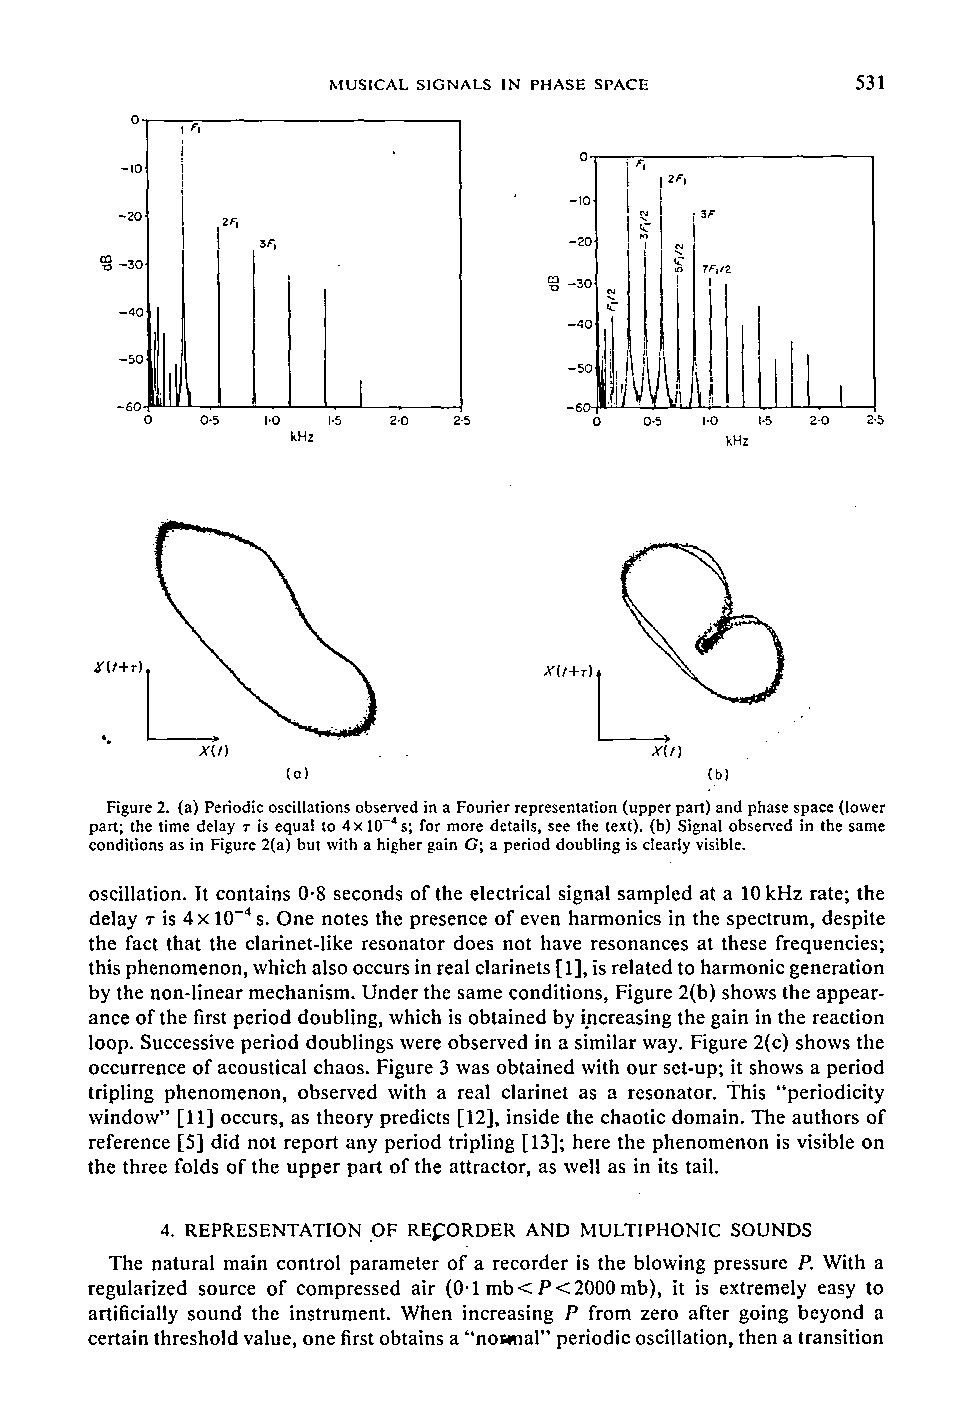
\includegraphics[trim=0 10.6cm 0 1.8cm, clip, width=0.75\textwidth]{report/Images/Gibiat_PhaseSpaceMusicalSignals_JSV_1988-p3.pdf}
    \caption{Démonstration du doublement de période due à l'augmentation du débit dans le bec de l'instrument. Tiré de \cite{gibiat_phase_1988}.}
    \label{fig:gibiat-double-period}
\end{figure}

\newpage

\fancypagestyle{plain}{plain}
 {\hypersetup{hidelinks} \printbibliography }


\end{document}
